\documentclass[conference]{IEEEtran}
\IEEEoverridecommandlockouts
% The preceding line is only needed to identify funding in the first footnote. If that is unneeded, please comment it out.
\usepackage{cite}
\usepackage{amsmath,amssymb,amsfonts}
\usepackage{algorithmic}
\usepackage{graphicx}
\usepackage{textcomp}
\usepackage{xcolor}
\usepackage{hyperref}
\usepackage{listings}
\usepackage{xcolor}

% Define Rust Language
\lstdefinelanguage{Rust}{
  basicstyle=\ttfamily,
  keywordstyle=\color{blue}\ttfamily,
  stringstyle=\color{red}\ttfamily,
  commentstyle=\color{green}\ttfamily,
  morecomment=[l]{//},
  morecomment=[s]{/*}{*/},
  morestring=[b]",
  morekeywords={
    as, break, const, continue, crate, else, enum, extern, false, fn, for,
    if, impl, in, let, loop, match, mod, move, mut, pub, ref, return, Self,
    self, static, struct, super, trait, true, type, unsafe, use, where, while
  },
}

\lstset{
  language=Rust,
  breaklines=true,
  captionpos=b,
  showstringspaces=false,
  basicstyle=\footnotesize\ttfamily,
  tabsize=2
}



\def\BibTeX{{\rm B\kern-.05em{\sc i\kern-.025em b}\kern-.08em
    T\kern-.1667em\lower.7ex\hbox{E}\kern-.125emX}}
\begin{document}
\title{Badlock: Static Reentrant Deadlock Detection for Rust via Taint Analysis}

\author{\IEEEauthorblockN{Liam Monninger}
\IEEEauthorblockA{\textit{Department of Computer and Information Science, SEAS} \\
\textit{University of Pennsylvania}\\
Philadelphia, PA, USA \\}}

\maketitle

\begin{abstract}
We present Badlock--a static analysis for detecting reentrant deadlocks in Rust programs: \href{https://github.com/many-branches/badlock}{https://github.com/many-branches/badlock}. We successfully analyzed simple Rust programs with and without deadlocks using Badlock. The primary challenges encountered were owed to the lack of a Robust Rust LLVM pass ecosystem. We would like to expand our work to successfully analyze more complex programs and include other forms of synchronization.
\end{abstract}

\begin{IEEEkeywords}
static analysis, deadlocks, rust, taint analysis
\end{IEEEkeywords}

\section{Introduction}

\subsection{Contributors}
Liam Monninger is solely responsible for this project. He implemented the \verb|lock-detection|, \verb|llvm-lock-detection|, all associated tests, an compiled all reports.

\subsection{Reentrant Deadlock}
\textbf{Definition (Reentrant Lock):} A reentrant lock is a synchronization mechanism that allows the same thread to acquire the same lock multiple times without causing a deadlock. 

\textbf{Definition (Reentrant Deadlock):} A reentrant deadlock is a specific type of deadlock situation in a concurrent system, where a thread attempts to acquire a lock that it already holds, but the lock acquisition rules of the system do not allow such re-acquisition, or the system's state leads to a deadlock.

Formally, let $T$ be a thread and $L$ be a lock. The situation can be described as follows:

\begin{itemize}
    \item $T$ holds $L$ (denoted as $Holds(T, L)$).
    \item $T$ requests $L$ again (denoted as $Requests(T, L)$).
    \item The system rules do not allow re-acquisition of $L$ by $T$ or cannot proceed without releasing $L$ which $T$ is unable to do, leading to a deadlock situation.
\end{itemize}

This situation can be modeled as a deadlock because $T$ is waiting for an event (the release of $L$) that can only happen by $T$ itself, creating a circular wait condition.

\subsection{Taint Analysis}
We modeled our taint analysis of reentrant deadlocks with the following datalog program.

\begin{lstlisting}[caption={Deadlock Taint Analysis Datalog Program}, label=lst:datalog]
@input
#[derive(Debug)]
pub struct Def(pub usize, pub usize);

@input
#[derive(Debug)]
pub struct UseVar(pub usize, pub usize);

@input
#[derive(Debug)]
pub struct Next(pub usize, pub usize);

@input
#[derive(Debug)]
pub struct Wrap(pub usize, pub usize);

@input
#[derive(Debug)]
pub struct Lock(pub usize, pub usize);

@input
#[derive(Debug)]
pub struct Release(pub usize, pub usize);


@output
#[derive(Debug)]
pub struct Kill(pub usize, pub usize);

@output
#[derive(Debug)]
pub struct In(pub usize, pub usize);

@output
#[derive(Debug)]
pub struct Out(pub usize, pub usize);

@output
#[derive(Debug)]
pub struct Deadlock(pub usize, pub usize, pub usize);

@output
#[derive(Debug)]
pub struct Edge(pub usize, pub usize, pub usize);

@output
#[derive(Debug)]
pub struct Path(pub usize, pub usize, pub usize);

// Reaching definitions
Kill(curr_inst, old_inst) <- Def(var, curr_inst), Def(var, old_inst);
Out(inst, inst) <- Def(_, inst);
Out(inst, def_inst) <- In(inst, def_inst), !Kill(inst, def_inst);
In(inst, def_inst) <- Out(prev_inst, def_inst), Next(prev_inst, inst);

// Deadlock taint
Edge(from_inst, to_inst, var) <- Def(var, from_inst), UseVar(var, to_inst), In(to_inst, from_inst);
Path(from_inst, to_inst, var) <- Lock(from_inst, var), Edge(from_inst, to_inst, var);
Path(prev, next, var) <- Path(prev, almost, var), !Release(almost, var), Edge(almost, next, var);
Deadlock(acquired_inst, var, reentrant_inst) <- Lock(reentrant_inst, var), Path(acquired_inst, reentrant_inst, var);
\end{lstlisting}

This program combines a standard reaching-definitions analysis with tainting and sanitizing of resource instructions based on \verb|Lock| and \verb|Release| facts.

We used the \verb|crepe| crate as solver, which implements a standard chaotic iteration with fact strata.

\subsection{Rust std::sync}
Rust's \verb|std::sync crate| is the standard crate for thread-based synchronization in the language. Resources can be wrapped in a \verb|Mutex| or \verb|RwLock| at any time. The lock for said mutex can then be acquired by calling \verb|.lock()| on the mutex and thread-safe object known as a guard is returned. The guard represents mutually exclusive access to the resource and can be released either by manually dropping the object or by relying on Rust's expression lifetimes to drop the resource.

\begin{lstlisting}[caption={Rust Mutex Example}, label=lst:rust_example]
use std::sync::Mutex;

fn main() {

    let mut x = 64;
    let mut safe_x = Mutex::new(x); // wrap resource
    
    // automatically drop guard
    {
        let mut guard = safe_x.lock().unwrap(); // acquire lock and get guard object
        *guard += 1;
        println!("Here is fine x: {}", *guard);
        // guard dopped here
    }

    
    // manually drop guard
    let mut no_deadlock = safe_x.lock().unwrap();
    *no_deadlock += 1;
    println!("Should also get here x: {}", *no_deadlock);
    drop(no_deadlock); // guard dropped here


}
\end{lstlisting}

In LLVM IR, manual drops and execution based drops are formed identically as calls to or invocations of \verb|core::ptr::drop_in_place|. This fact simplified our implementation of the static pass.

Ultimately, we were able to successfully extract the necessary \verb|Lock| and \verb|Release| facts from the Rust \verb|std::sync crate| via demangling invocation and calls to know functions. These were:

\begin{itemize}
    \item \verb|std::sync::Mutex::new|
    \subitem \verb|Def|
    \subitem \verb|UseVar|
    \item \verb|std::sync::Mutex::lock|
    \subitem \verb|Lock|
    \subitem \verb|Def|
    \subitem \verb|UseVar|
    \item \verb|core::ptr::drop_in_place<std::sync::MutexGuard>|
    \subitem \verb|Release|
    \subitem \verb|Def|
    \subitem \verb|UseVar|
\end{itemize}

\section{Badlock}
We implemented our analysis software as a Rust workspace we call badlock. Badlock was evaluated as sound against a set of simple programs detailed below.

\begin{figure}[ht]
    \centering
    \fbox{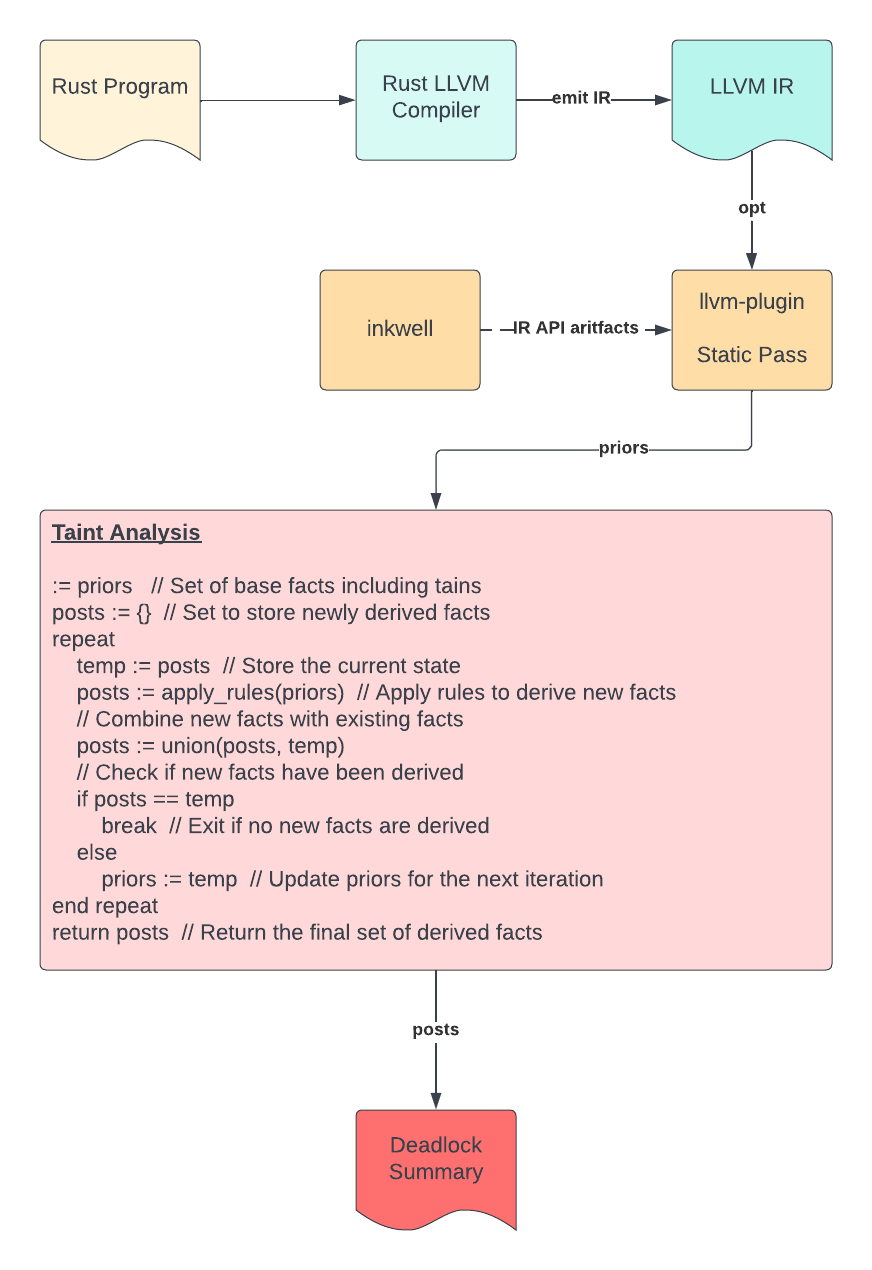
\includegraphics[width=0.5\textwidth]{./rsc/Badlock.png}}
    \caption{High-level diagram of Badlock.}
    \label{fig:badlock_sys}
\end{figure}

\subsection{Evaluation}
We are currently capable of detecting deadlocks in the following simple programs. Programs of this form were defined as the original POC.

\subsubsection{No Deadlock}
We were able to successfully analyzing clearly non-deadlocking Rust programs wherein no lock is ever acquired. The below is an example of a passing program.

\begin{lstlisting}[caption={Program Without a Deadlock}, label=lst:rust_example]
fn main(){

    let a = 0;
    for i in 0..10 {
        let b = a + i;
        println!("{}", b);
    }
    
}
\end{lstlisting}

\subsubsection{Simple Deadlock}
We successfully analyzed simple deadlocking programs which use std::sync::Mutex such as the following.

\begin{lstlisting}[caption={Program With A Simple Deadlock}, label=lst:rust_example]
use std::sync::Mutex;

fn main() {

    let mut safe_x = Mutex::new(64);
    
    let mut guard = safe_x.lock().unwrap();
    *guard += 1;
    println!("Here is fine x: {}", *guard);

    let mut deadlock = safe_x.lock().unwrap();
    *deadlock += 1;
    println!("Should never get here x: {}", *deadlock);

}
\end{lstlisting}

\subsubsection{Safe Lock Acquisition}
We successfully analyzed simple programs where locks are acquired and locked in a manner preventing reentrancy. Notably, we successfully analyzed the implicit lock releases that occur when a Rust lifetime ends.

\begin{lstlisting}[caption={Program With Safe Lock Acquisition}, label=lst:rust_example]
use std::sync::Mutex;

fn main() {

    let mut x = 64;
    let mut safe_x = Mutex::new(x);
    
    {
        let mut guard = safe_x.lock().unwrap();
        *guard += 1;
        println!("Here is fine x: {}", *guard);
    }

    {
        let mut no_deadlock = safe_x.lock().unwrap();
        *no_deadlock += 1;
        println!("Should also get here x: {}", *no_deadlock);
    }

}
\end{lstlisting}

\section{Conclusion}
In developing Badlock, we implemented a simple and modular taint-analysis for reentrant deadlocks. We then provided a proof of concept implementation of a static pass which soundly uses this analysis to accurately detect deadlocks encountered in the usage of \verb|std::sync::Mutex|. 

There is much work to be done to further research edge cases and make Badlock's static pass more robust. We, additionally, hope to expand the project to include other Rust synchronization primitives, such as \verb|std::sync::RwLock| crates such as \verb|tokio::sync|.

We, however, recognize that the Rust ecosystem for developing LLVM static passes is underdeveloped. We anticipate that further progress on Badlock may best be empowered by contributing improvements to existing crates.

Finally, we would eventually like to expand our work to include other kinds of concurrency bugs, perhaps via hybrid-analysis.

\begin{thebibliography}{00}
    \bibitem{b1} Crepe, A Datalog-Inspired Language for Rust. Available at: \url{https://github.com/ekzhang/crepe}
    \bibitem{b2} LLVM Plugin for Rust. Available at: \url{https://github.com/jamesmth/llvm-plugin-rs}
    \bibitem{b3} Inkwell, a Rust Wrapper for LLVM's C++ API. Available at: \url{https://github.com/TheDan64/inkwell}
\end{thebibliography}
    

\end{document}
